\documentclass[9pt,twocolumn,twoside]{pnas-new}
% Use the lineno option to display guide line numbers if required.

\articletype{Social Sciences}%%%% Article topic/classification
\templatetype{pnasresearcharticle} % Choose template
% {pnasresearcharticle} = Template for a two-column research article
% {pnasmathematics} %= Template for a one-column mathematics article
% {pnasinvited} %= Template for a PNAS invited submission

% Figure search path — assumes manuscript.tex lives next to the Paper_Figures
% folder (i.e., /Users/elanbarenholtz/Projects/lrtia/paper/). Adjust if not.
\graphicspath{{Paper_Figures/}}

\begin{document}

\title{Universal power law decay of sequential influence in human language generation}

% Use letters for affiliations, numbers to show equal authorship (if applicable) and to indicate the corresponding author
\author[a,1]{Elan Barenholtz}

\affil[a]{Department of Psychology and Center for Complex Systems, Florida Atlantic University, 7777 Glades Rd, Boca Raton, FL 33431}

% Please give the surname of the lead author for the running footer
\leadauthor{Barenholtz}

% Please add a significance statement to explain the relevance of your work
\significancestatement{Coherent language requires that earlier content continue to shape later content across sentences and discourse. Yet how this influence decays as a function of distance, and what it reveals about cognition, has remained largely uncharacterized. We show that human language production across 8 languages, 6 language families, and both written and spoken modalities encodes a universal power law decay of contextual influence. The exponent is invariant across typologically diverse languages, robust across two probe models, and converges with independent measurements from memory retrieval research. AI-generated text shows a categorically different pattern, with coherence collapsing at distances where human text retains influence. We propose this universal form reflects the dynamics of autoregressive generation, with implications for linguistic theory and memory.}

% Please include corresponding author, author contribution and author declaration information
\authorcontributions{E.B. designed research, performed research, analyzed data, and wrote the paper.}

\authordeclaration{The author declares no competing interests.}

\correspondingauthor{\textsuperscript{1}To whom correspondence should be addressed. E-mail: \href{mailto:ebarenholtz@fau.edu}{ebarenholtz@fau.edu}}

% At least three keywords are required at submission. Please provide three to five keywords, separated by the pipe symbol.
\keywords{language production $|$ autoregressive generation $|$ power law $|$ cross-linguistic invariance $|$ computational linguistics}

\begin{abstract}
How contextual influence decays during human language production has remained largely uncharacterized despite its centrality to coherent discourse. We report a universal power law of sequential influence decay: the marginal predictive contribution of prior context falls off as $d^{-\alpha}$, with exponents between $-0.69$ and $-0.88$ across written and spoken language spanning 8 languages and 6 language families. The pattern is robust across two independent probe models (Llama-3-8B mean $\alpha = -0.78$; Mistral-7B mean $\alpha = -0.74$ for well-fitted conditions). Formal model comparison by AIC and BIC selects the power law over exponential, logarithmic, and stretched exponential alternatives in 75\% of cases; the exponential form is never selected by the better-calibrated probe. Beyond the exponent, human language maintains substantial absolute coherence at 30--50 tokens (0.05--0.24 in corrected marginal units), where AI-generated text has already collapsed to the floor (0.03--0.05); this dissociation holds across English, Chinese, and Turkish in matched comparisons. The exponent range converges with two independent memory measurements made by entirely different methods: Anderson and Schooler's environmental information recurrence statistics ($\alpha \approx -0.77$) and Kahana et al.'s associative decay in free recall ($\alpha \approx -0.82$). We propose that the universal power law reflects the dynamics of autoregressive generation in human language production: a scale-free chaining process in which each generative step compresses a comparable proportion of prior influence. The form provides a mechanistic basis for the observed cross-linguistic invariance and offers direct empirical evidence for sequential generative accounts of language production over alternatives positing non-sequential hierarchical computation as its engine.
\end{abstract}

\dates{This manuscript was compiled on \today}
\doi{\url{www.pnas.org/cgi/doi/10.1073/pnas.XXXXXXXXXX}}

\maketitle
\thispagestyle{firststyle}
\ifthenelse{\boolean{shortarticle}}{\ifthenelse{\boolean{singlecolumn}}{\abscontentformatted}{\abscontent}}{}

\Firstpage
%The \Firstpage command is used to format the first page text column size. The same size will be maintained for subsequent paragraph until the \Endparasplit or \Parasplit command is encountered.

\dropcap{C}oherent extended language is a remarkable achievement. The fourth sentence of a paragraph is constrained by the first three; the choice of pronoun in clause five depends on what was introduced in clause one; a word produced now must remain coherent with words produced minutes ago. This ongoing constraint---the influence of prior content on current production---is what makes language coherent rather than locally fluent but globally incoherent. Yet how it operates as a function of distance, and what it reveals about the cognitive processes underlying production, has remained largely uncharacterized. Existing measures of linguistic dependency typically focus on specific phenomena such as syntactic agreement or anaphoric reference, leaving the broader question of how influence decays across the generative sequence largely unaddressed.

The question bears directly on theoretical accounts of language production. Hierarchical-computation accounts, exemplified by the generative grammar tradition \cite{chomsky1995minimalist}, hold that production is driven by abstract structural operations over phrasal and clausal units, with surface-level sequential dependencies emerging as downstream consequences. Autoregressive accounts hold the opposite: language is generated token by token, each token conditioned on prior tokens, with apparent hierarchical structure emerging from this sequential process rather than driving it. The two views make distinguishable predictions about the shape of the decay curve. Hierarchical accounts predict dependencies organized around hierarchical units---qualitative transitions in the curve at the corresponding distances. Autoregressive accounts predict a specific functional form: scale-free power law decay reflecting the proportional compression that occurs at each generative step.

Here we develop a general method for measuring this decay and use it to adjudicate between the two accounts. Using large language models as measuring instruments, we quantify how much prior context continues to influence current language as a function of distance. The method is token-level, language-agnostic, and requires no syntactic or semantic annotation. We apply it to human-generated text and speech across 8 languages and 6 language families spanning typologically diverse linguistic structures, and to matched AI-generated text across 3 languages. We find a universal power law decay in human language production, with exponents that cluster in a characteristic range across modalities and typology, that is robust to probe-model choice, and that is categorically distinct from the pattern observed in AI-generated text. The same exponent range has been reported, by completely different methods, in two independent memory retrieval studies separated by a decade \cite{anderson1991reflections,kahana2002age}. We argue that the universal form is the signature of autoregressive generation in human language production.

\Endparasplit
%The \Endparasplit command is used to end the formatting of the text column size that was set by the \Firstpage command. This will restore the default column size for the subsequent text.

% =============================================================================
% RESULTS
% =============================================================================

\section*{Results}

\subsection*{A token-level measure of sequential influence}

We developed a method for measuring how much prior context influences current language production, independent of language, modality, or genre. Using a large language model as a probe---not as the object of study---we revealed context one token at a time and measured the perplexity of a fixed target region at each context length. To isolate the contribution of sequential structure from the distributional calibration benefit a model gains from any tokens regardless of order, we subtracted a shuffled-context baseline in which the same tokens were presented in random order. The corrected marginal at distance $d$ is the difference between intact-context and shuffled-context perplexity reduction at that distance: $\Delta_d = m^{\text{intact}}_d - m^{\text{shuffled}}_d$, where $m_d = \text{perplexity}_{d-1} - \text{perplexity}_d$. This quantity measures what the sequential structure of prior content, as distinct from its distributional properties, contributes to predicting current content.

The shuffled-context control is essential. Without it, raw perplexity reduction conflates two distinct effects: the model's calibration to the input distribution (which improves with more tokens regardless of order) and the contribution of sequential coherence (which requires order). The corrected measure isolates the latter. We fit power law, exponential, stretched exponential, and logarithmic functions to the corrected marginal curve via nonlinear least squares on log-transformed data, and compared models using AIC and BIC. All analyses were conducted independently with two probe models---Llama-3-8B \cite{llama3} and Mistral-7B \cite{mistral7b}---to assess robustness to probe-specific properties.

\subsection*{Power law decay is the universal functional form}

Across 16 dataset--probe combinations spanning 8 languages, 6 language families, written and spoken modalities, and two probe models, the power law was selected as the best-fitting functional form by both AIC and BIC in 12 of 16 cases (75\%; \emph{SI Appendix}, Table~S2). Linear decay was never selected, confirming that the decay is robustly nonlinear in all conditions. The exponential form was not selected by Llama-3-8B for any dataset; Llama-3-8B selected the power law for every dataset except Korean Wikipedia, which was best fit by a stretched exponential---a two-parameter generalization of the power law that preserves the scale-free property. The two exponential wins across both models correspond to Finnish and Chinese Wikipedia under Mistral-7B, the two conditions where Mistral showed the weakest overall fit, consistent with functional-form instability under poor probe calibration rather than genuine exponential structure.

The form has a specific theoretical implication. An exponential decay implies a characteristic scale---a distance beyond which prior content becomes effectively unavailable---consistent with discrete capacity-limited processing. A power law has no characteristic scale: the influence of prior content decays steeply at first but retains a heavy tail at long distances, and the proportional reduction per unit distance is constant. The universal preference for power law over exponential, particularly under the better-calibrated probe, indicates that sequential influence in human language production has no characteristic cutoff. The same conclusion follows from the absence of any qualitative transition in the curve. If production were governed by processes operating over discrete units of fixed scale---working memory chunks \cite{cowan2001magical}, syntactic phrases, or clausal units---the curve should change character at the corresponding distances. We observe no such transition. The power law is a single unbroken component across the full 1--100 token range in every corpus tested, and formal model comparison does not select any two-component form.

\subsection*{Cross-linguistic and cross-modal invariance}

The corrected influence-decay exponent clusters in a characteristic range across typologically diverse human language (Table~\ref{tab:exponents}). Llama-3-8B yields exponents between $-0.70$ and $-0.88$ (mean $-0.78$, SD $= 0.06$). Mistral-7B yields exponents between $-0.61$ and $-0.82$ for well-fitted conditions (mean $-0.74$, SD $= 0.05$). The two probes agree most closely for French spoken narrative (Llama $-0.70$, Mistral $-0.69$) and converge within 0.15 for all well-fitted conditions. Inter-model divergence is largest for Arabic and Finnish, the two languages most underrepresented in Mistral's training data, consistent with the interpretation that residual variance reflects probe calibration quality rather than genuine cross-linguistic differences in the exponent.

The range spans six unrelated language families: Sino-Tibetan, Japonic, Koreanic, Turkic, Afro-Asiatic, Uralic, Germanic, and Romance. These languages encompass verb-final, verb-initial, and verb-medial word orders; isolating, agglutinative, and fusional morphological types; tonal and non-tonal phonology; left-to-right and right-to-left writing systems; and both written and spoken production modes. The characteristic exponent range is preserved across this typological diversity. If the decay reflected properties of specific syntactic structures, exponents should vary systematically with typology. They do not. The same characteristic decay form appears across languages with fundamentally different hierarchical organization, suggesting that the underlying mechanism operates similarly regardless of the specific linguistic structure being produced (Fig.~\ref{fig:cross-linguistic}).

\subsection*{Human language sustains long-range coherence that AI text does not}

Beyond the exponent, the absolute magnitude of the corrected influence signal reveals a qualitative difference between human and AI text that exponent comparisons alone do not capture (Fig.~\ref{fig:human-vs-ai}). At 30--50 tokens---roughly 20--30 words, or 15--20 seconds of conversational speech---non-English human text maintains corrected marginal values between 0.05 and 0.24. English spoken text (Buckeye \cite{pitt2005buckeye}) shows the highest long-range coherence in the dataset at 0.237; French spoken narrative shows 0.156; non-English Wikipedia corpora range from 0.047 (Finnish) to 0.203 (Chinese). AI-generated text (Claude Sonnet, matched by topic and language) shows long-range values of 0.029--0.052---a factor of 3--6 lower than matched human text in the same languages. At 30--50 tokens, AI coherence influence has effectively collapsed to the floor. The dissociation in absolute long-range coherence holds across all three matched language comparisons (English, Chinese, Turkish) and both probe models. AI exponents are also steeper than human exponents in 5 of 6 probe--language combinations (\emph{SI Appendix}, Table~S1).

The dissociation is theoretically informative. AI language models are explicitly autoregressive systems, generating text token by token with each token conditioned on prior tokens. Yet they fail to reproduce the human pattern. The same scale-free shape is preserved---suggesting that the power-law form is generic to deep chaining processes---but the human system maintains influence over a longer effective chain than current artificial systems do. The mechanistic basis of this difference remains an open question, with candidates including the depth of compression performed at each generative step, the recursive coupling between generated content and the structures generating it, and the role of non-linguistic representational systems that may extend the effective range of coherence-supporting information.

% =============================================================================
% TABLE 1 — full-width table because it has 8 columns
% =============================================================================

\begin{table*}[t!]
\centering
\caption{Cross-linguistic and cross-modal influence-decay exponents. Probe correlation $r$ on log-log fit; values $|r| < 0.80$ indicate poor probe calibration and are excluded from the Mistral summary statistics.}
\label{tab:exponents}
\begin{tabular*}{\textwidth}{@{\extracolsep{\fill}}llllrrrr@{}}
\toprule
Dataset & Language & Family & Modality & Llama $\alpha$ & Llama $r$ & Mistral $\alpha$ & Mistral $r$ \\
\midrule
Chinese Wiki  & Chinese  & Sino-Tibetan & Written & $-0.77$ & $-0.97$ & $-0.82$ & $-0.97$ \\
Japanese Wiki & Japanese & Japonic      & Written & $-0.81$ & $-0.95$ & $-0.72$ & $-0.95$ \\
Korean Wiki   & Korean   & Koreanic     & Written & $-0.73$ & $-0.96$ & $-0.69$ & $-0.96$ \\
Turkish Wiki  & Turkish  & Turkic       & Written & $-0.88$ & $-0.97$ & $-0.79$ & $-0.95$ \\
Arabic Wiki   & Arabic   & Afro-Asiatic & Written & $-0.79$ & $-0.95$ & $-0.61$ & $-0.66$ \\
Finnish Wiki  & Finnish  & Uralic       & Written & $-0.77$ & $-0.91$ & $-0.56$ & $-0.50$ \\
Buckeye       & English  & Germanic     & Spoken  & $-0.87$ & $-0.93$ & $-0.73$ & $-0.93$ \\
French Oral   & French   & Romance      & Spoken  & $-0.70$ & $-0.89$ & $-0.69$ & $-0.85$ \\
\bottomrule
\end{tabular*}
\addtabletext{Llama-3-8B: mean $-0.78$, SD $0.06$, range $[-0.70, -0.88]$. Mistral-7B (well-fit only): mean $-0.74$, SD $0.05$.}
\end{table*}

% =============================================================================
% DISCUSSION
% =============================================================================

\section*{Discussion}

We report a universal power law of sequential influence decay in human language production, robust across 8 languages, 6 language families, written and spoken modalities, and two independent probe models. The power law form is preferred over exponential alternatives by formal model comparison, with the exponential form never selected by the better-calibrated probe. Human text maintains substantial long-range coherence at 30--50 tokens that AI-generated text does not. The exponent range converges with independent measurements from memory retrieval research conducted by completely different methods over three decades.

\subsection*{Autoregressive generation as the underlying mechanism}

The empirical pattern places three constraints on theoretical accounts of language production. First, the universal preference for power law over exponential decay, with no characteristic scale, is inconsistent with accounts that posit discrete processing units of fixed capacity---working memory buffers, phrasal units, clausal units---as the locus of sequential dependency. Such accounts predict a characteristic scale at which decay dynamics qualitatively change; the data show no such scale. Second, the cross-linguistic invariance of the exponent across typologically diverse languages constrains accounts in which surface-level dependency patterns are downstream consequences of language-specific hierarchical structures. If hierarchical structure varied across languages while the decay pattern remained constant, the relationship between hierarchical structure and surface decay would be considerably more attenuated than such accounts typically assume. Third, the dissociation from AI-generated text rules out accounts in which the human pattern emerges directly from the statistical properties of token sequences: AI systems trained on human text do not reproduce it.

We propose that the empirical pattern is most parsimoniously interpreted as the signature of autoregressive generation in human language production. In an autoregressive system, each generated token is produced from the current state and then absorbed into it. The state at time $t$ already expresses the integrated influence of every prior token. Past tokens do not need to be retrieved from a separate store to exert influence on current generation; they exert influence by having shaped the trajectory that produced the current state.

This forces a reframing of what the decay curve measures. The corrected marginal at distance $d$ is not the rate at which past tokens fade from any buffer. It is the rate at which the marginal information they contribute, beyond what is already encoded in nearer tokens, declines with distance. Tokens at distance $d$ have had their contribution chained forward through $d$ generative steps. At each step, what they contributed was absorbed into the produced token, which was then itself absorbed into the next. Recent tokens are not more influential because they have decayed less; they are more influential because they carry forward, in their own current presence, the cumulative contribution of everything before them. Older tokens add diminishing marginal information because more of what they contributed is already represented redundantly in the chain that followed.

The power law is the signature of this process being scale-free. Moving from $d$ to $d+1$ costs the same fraction of remaining influence whether $d$ is 10 or 100. This is what one expects when each chaining step compresses comparable proportions of remaining information, and the trajectory has no scale at which the compression process changes character. Exponential decay, by contrast, would correspond to accelerating compression, with each step costing a larger fraction of remaining influence---a process with a characteristic clearance scale. The cross-linguistic stability further supports the interpretation: if the power law reflected properties of any specific linguistic structure, exponents should vary with typology, but they do not. The exponent reflects the chaining process itself, which operates the same way regardless of what is being chained. The dissociation from current AI systems indicates that artificial autoregressive systems share the scale-free shape that any sufficiently deep chaining process should produce, but do not maintain influence over as long a chain. The mechanistic basis of that difference is an open question and a productive direction for future work.

\subsection*{Convergence with memory retrieval research}

The convergence of the production-side exponent range with two independent measurements from memory retrieval research is striking (Fig.~\ref{fig:convergence}). Anderson and Schooler \cite{anderson1991reflections}, examining the recurrence statistics of information demand in natural environments, reported a power law with exponent of approximately $-0.77$. Kahana et al. \cite{kahana2002age}, examining associative decay in free recall, reported a forward exponent of approximately $-0.82$ for younger adults. Both measurements were made with completely different methods on completely different data, and involve no language model. All three traditions converge on a characteristic exponent range. The same form has been documented for forgetting more broadly \cite{wixted1991form,rubin1996one}.

On the autoregressive account, this convergence is interpretable. Language production samples the influence of past tokens on next-token generation; environmental statistics sample the recurrence structure of experience that production is tuned to; free recall samples the system's ability to regenerate past states from prior experience. Whether these traditions tap a common underlying process or merely produce similar exponents through distinct mechanisms is a question the present data motivate but do not settle. Direct empirical investigation in non-linguistic sequential domains will be required to determine whether autoregressive generation operates as a domain-general principle of biological cognition or whether the convergence reflects shared but mechanistically distinct constraints across paradigms.

\subsection*{Limitations and outlook}

Several limitations should be noted. The probe-model approach measures predictability as a proxy for generative influence, and specific exponent values are somewhat probe-dependent, as the inter-model comparison demonstrates; what is robust across probes is the power law form, the categorical separation from AI text, and the overall human exponent range. The Buckeye and French Oral Narrative spoken corpora are limited in size relative to the Wikipedia corpora. The AI comparison uses a single AI system and should be extended to multiple systems, including those with explicit multimodal grounding. The autoregressive-generation interpretation, while parsimonious given the present results, is a framework for explaining the empirical pattern rather than a directly tested mechanism; direct tests in non-linguistic sequential domains (music improvisation, motor sequences, drawing, gesture) are required to determine whether the framework extends beyond language.

These findings establish that human language production exhibits the universal mathematical signature of autoregressive generation, providing direct empirical support for sequential generative accounts of language production over alternatives that posit non-sequential hierarchical computation as the underlying engine. The convergence with memory retrieval measurements suggests these traditions may share common ground worth exploring directly. Whether autoregressive generation operates as a domain-general principle of biological cognition, and whether it offers a productive reframing of memory phenomena more broadly, are questions for future work.

% =============================================================================
% FIGURES
% =============================================================================
% PNAS allows ~4 graphical elements in main text for a 6-page Research Report.
% Plan: 1 table + 3 figures = 4 elements.
%
% MAIN TEXT:
%   Table 1                  — cross-linguistic exponents (above)
%   Figure 1 (cross-ling.)   — fig3_crosslingual_convergence.png
%   Figure 2 (human vs AI)   — fig1_human_vs_ai_curves.png
%   Figure 3 (convergence)   — fig6_grand_summary.png
%
% PUSHED TO SI:
%   Fig S1 — fig2_functional_form.png       (power law vs alternatives)
%   Fig S2 — fig4_per_speaker.png            (per-speaker Buckeye)
%   Fig S3 — fig5_absolute_magnitude.png     (absolute coherence magnitudes)
%   Tab S1 — absolute coherence magnitudes
%   Tab S2 — functional-form AIC/BIC winners
% =============================================================================

\begin{figure*}[t!]
\centering
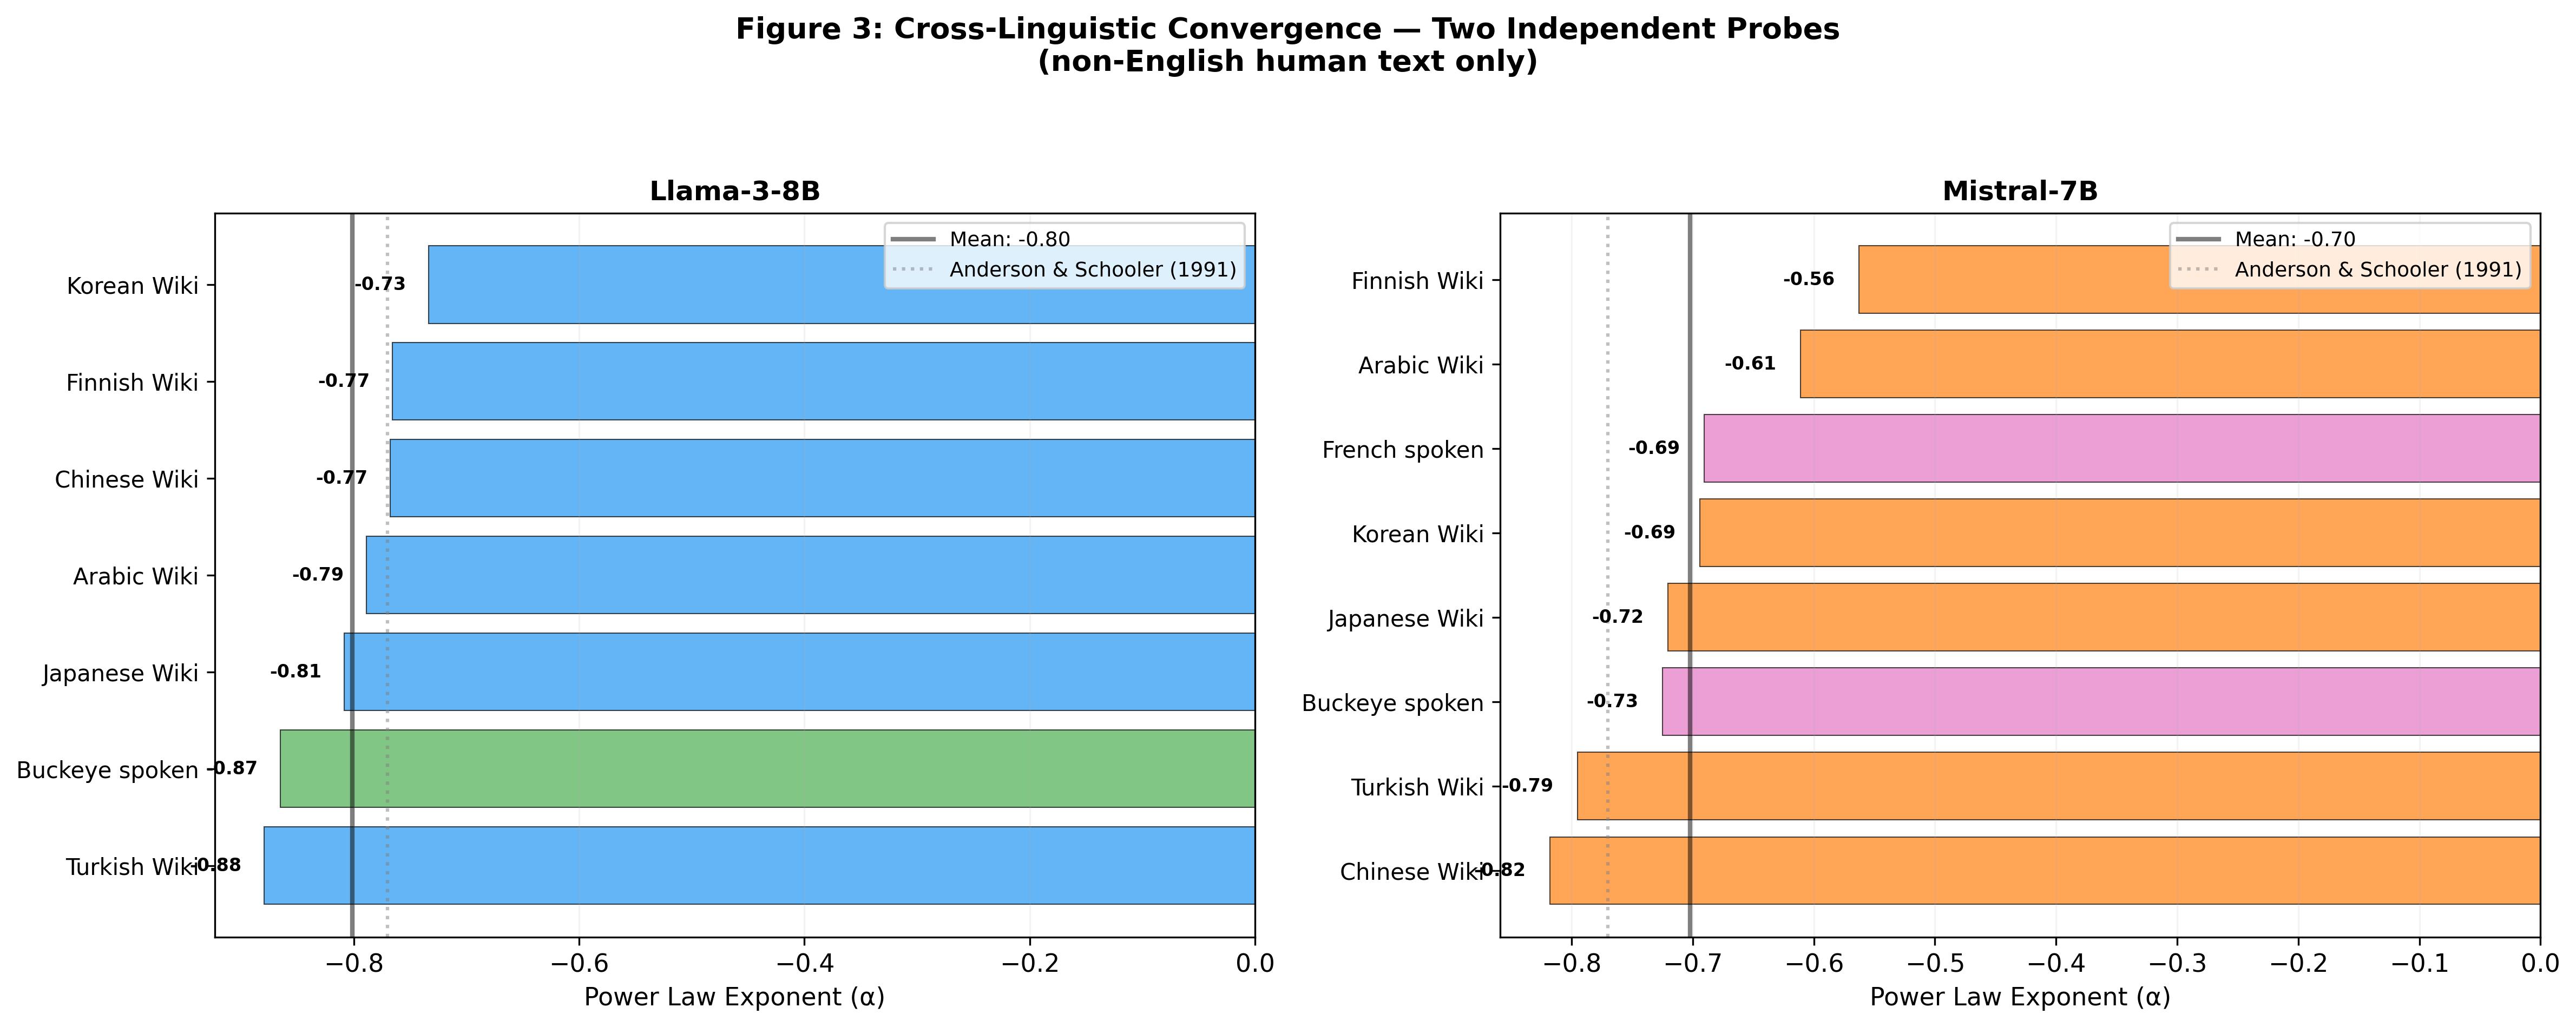
\includegraphics[width=.85\linewidth]{fig3_crosslingual_convergence.png}
\caption{Cross-linguistic convergence on a single influence-decay exponent. Corrected marginal influence as a function of token distance for 8 languages spanning 6 language families and two modalities (Wikipedia written corpora and Buckeye / French Oral spoken corpora), measured with two independent probe models. Power-law fits in log-log coordinates. The characteristic exponent range $-0.69$ to $-0.88$ is preserved across typology and modality.}
\label{fig:cross-linguistic}
\end{figure*}

\begin{figure*}[t!]
\centering
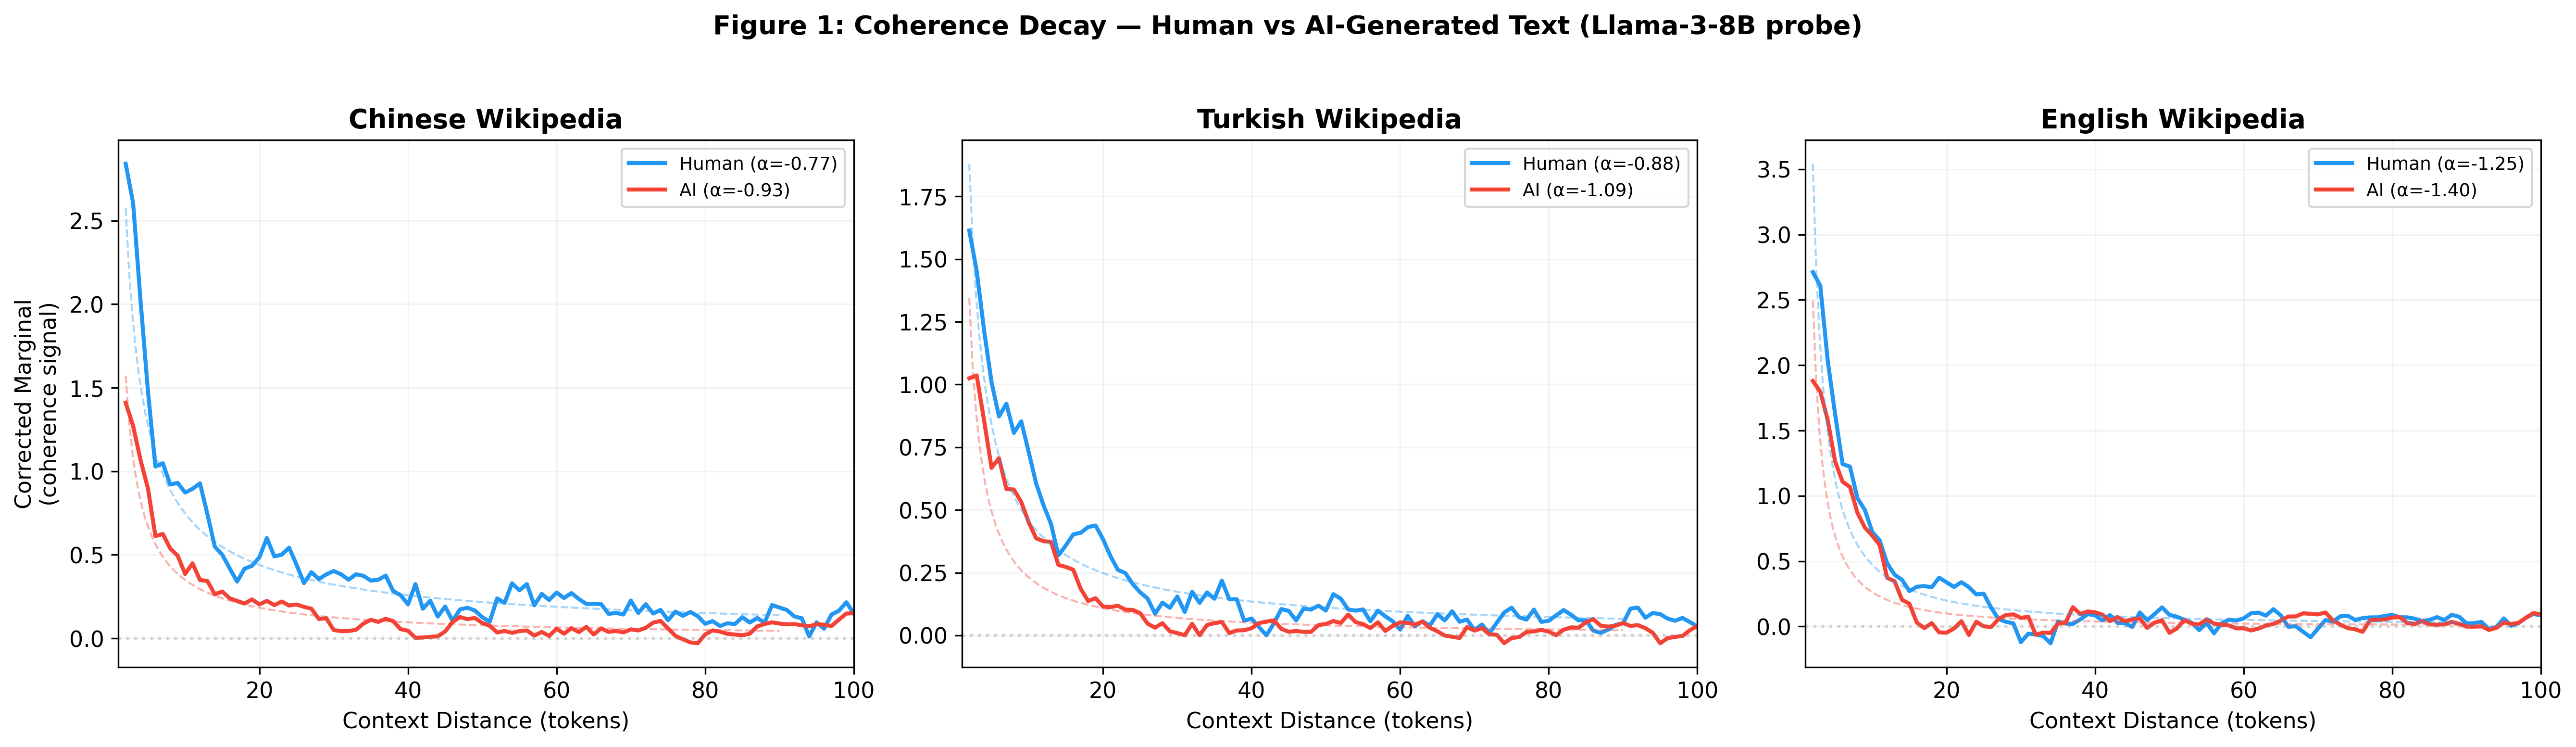
\includegraphics[width=.85\linewidth]{fig1_human_vs_ai_curves.png}
\caption{Human language sustains long-range coherence that AI-generated text does not. Log-log plots of corrected marginal vs.\ distance for representative human corpora and matched AI-generated text (Claude Sonnet, English / Chinese / Turkish). Human curves remain well above the floor through 30--50 tokens; AI curves collapse to the floor at the same distances. Pattern holds across all three matched language comparisons and both probe models.}
\label{fig:human-vs-ai}
\end{figure*}

\begin{figure*}[t!]
\centering
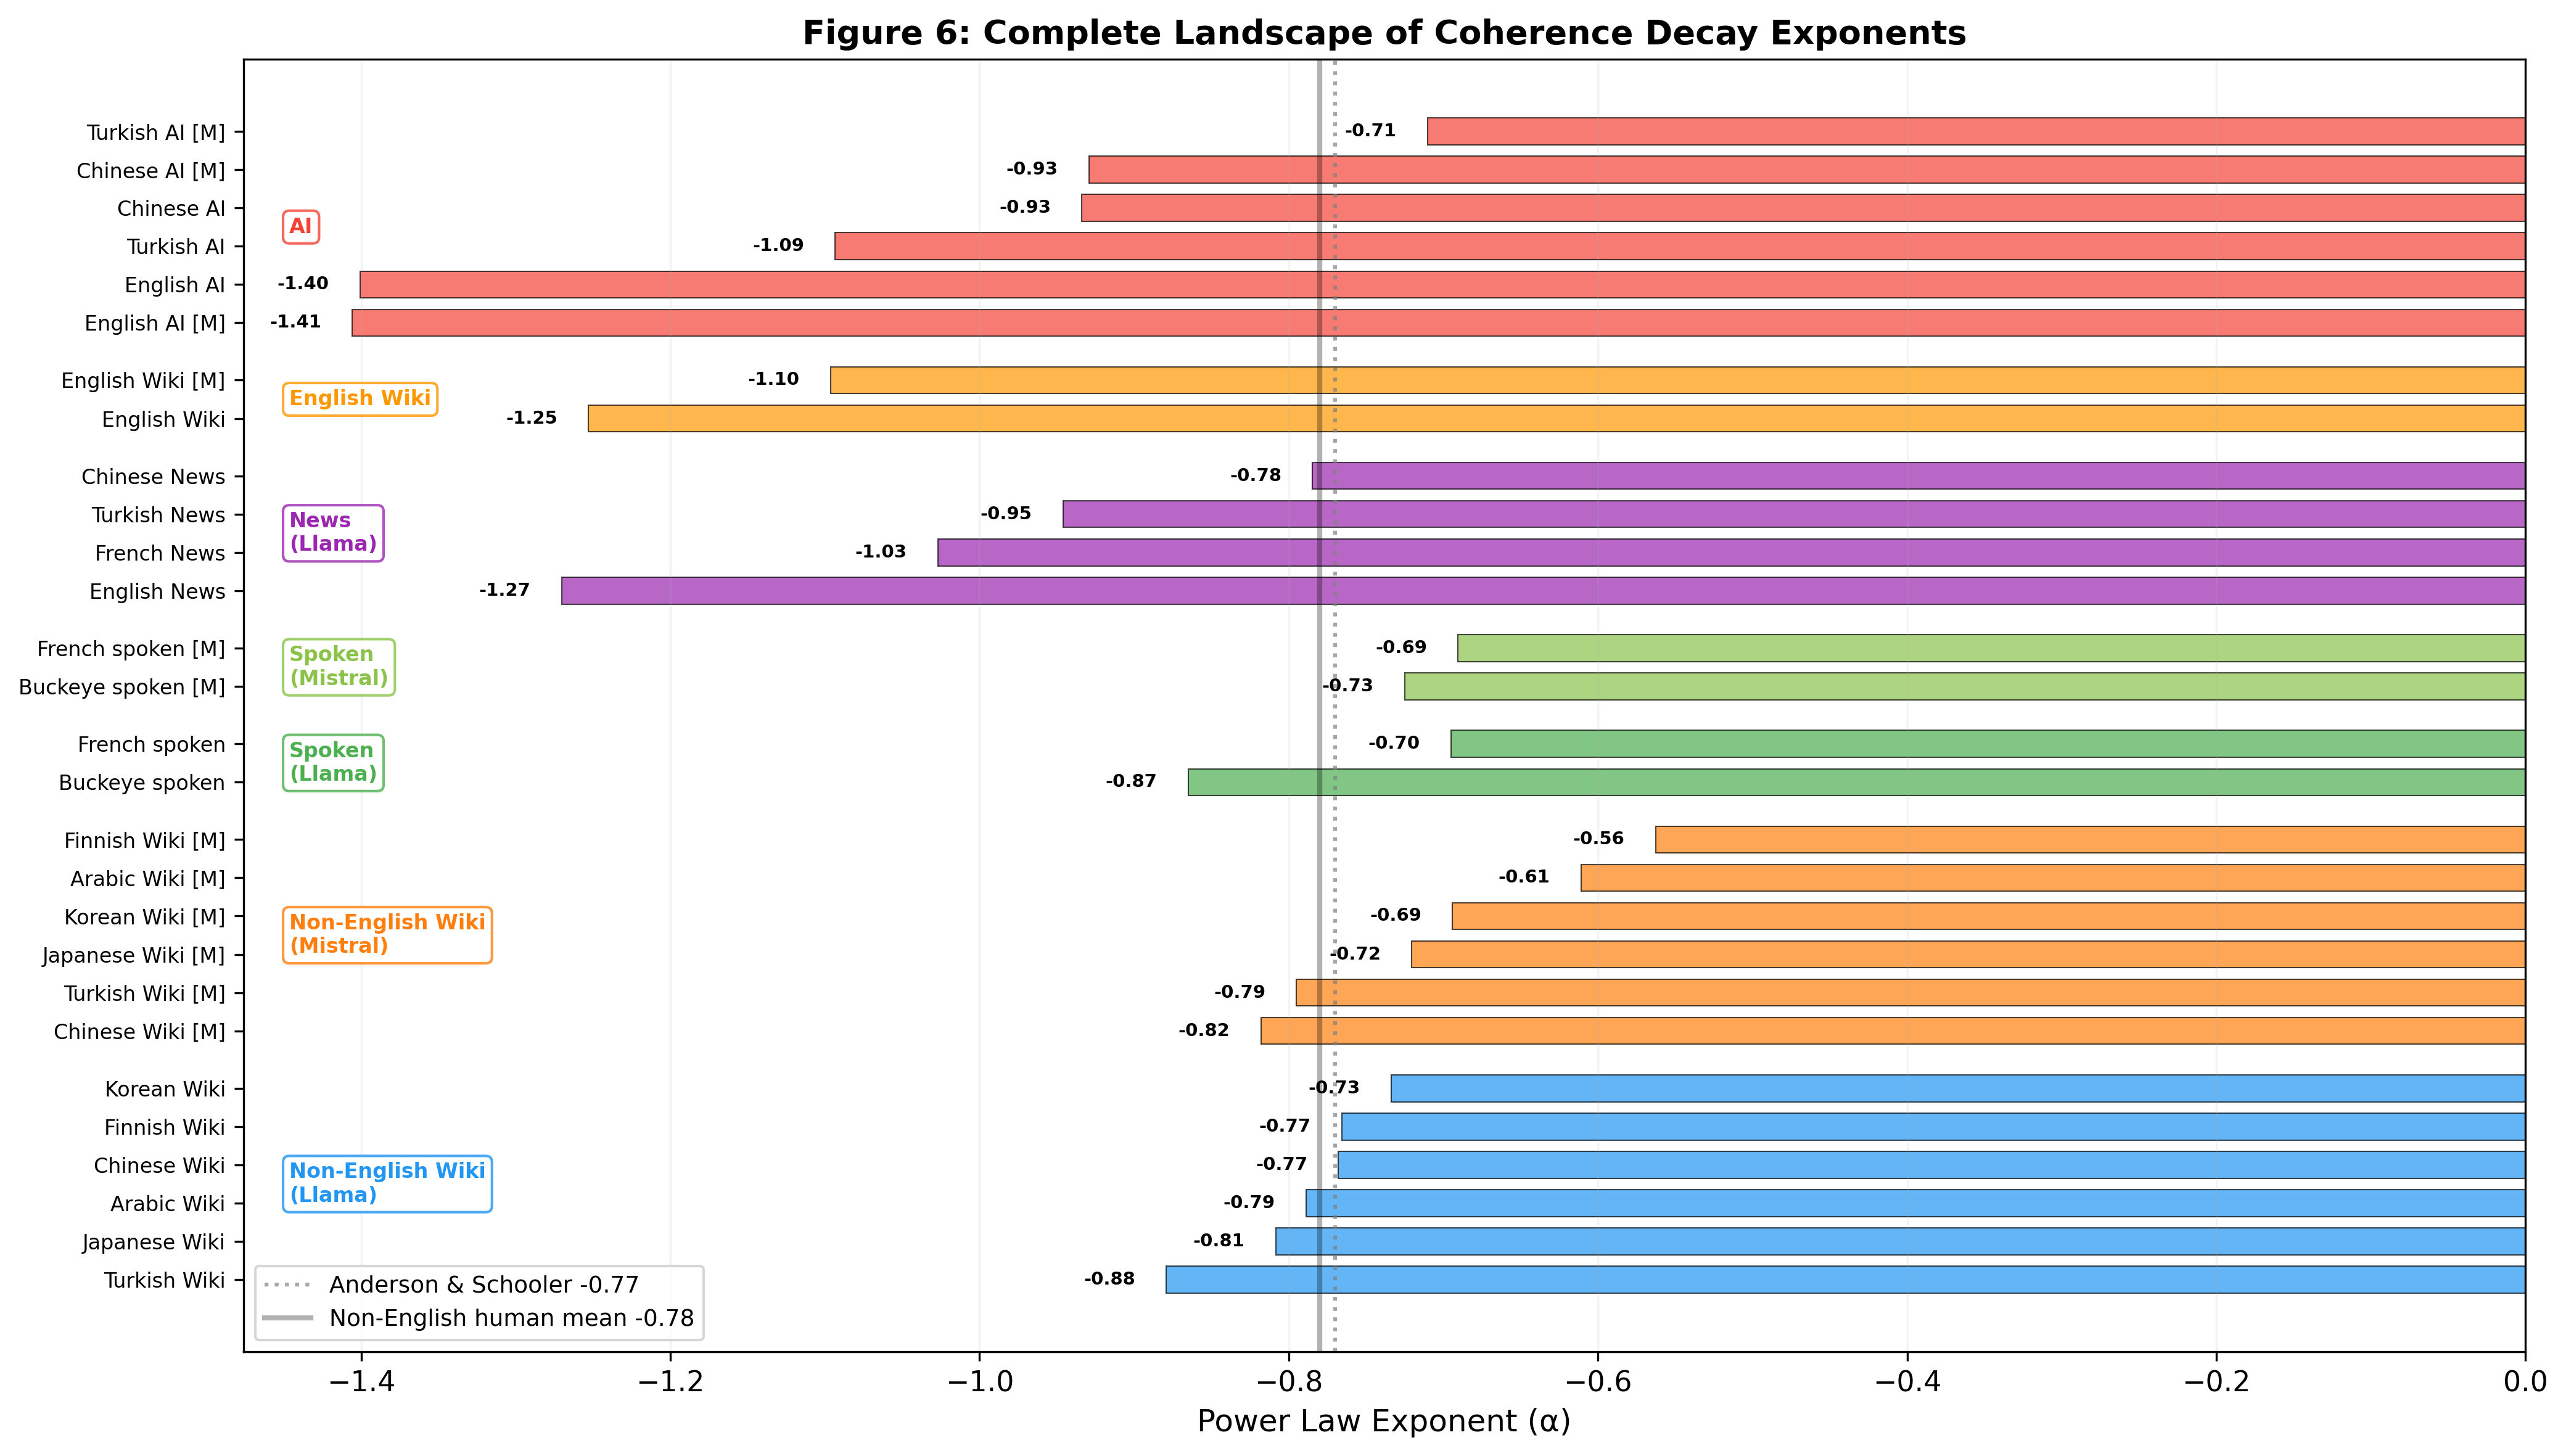
\includegraphics[width=.85\linewidth]{fig6_grand_summary.png}
\caption{Convergence of the production-side exponent range with independent memory-retrieval measurements. Exponents from the present study (Llama-3-8B and Mistral-7B, each dataset a point), Anderson \& Schooler's (1991) environmental information recurrence statistics ($\alpha \approx -0.77$), and Kahana et al.'s (2002) lag-CRP forward decay in free recall ($\alpha \approx -0.82$). Three traditions, three methods, three decades, one exponent range.}
\label{fig:convergence}
\end{figure*}

% =============================================================================
% MATERIALS AND METHODS (PNAS short M&M)
% =============================================================================

\matmethods{

\subsection*{Corpora}
Written corpora comprised Wikipedia articles in six languages (Chinese, Japanese, Korean, Turkish, Arabic, Finnish; 60 articles per language, drawn from current Wikipedia dumps). Spoken corpora comprised the Buckeye Corpus of Conversational Speech \cite{pitt2005buckeye} (26 speakers, spontaneous sociolinguistic interviews, English; interviewer turns excluded) and the French Oral Narrative Corpus (Queen's University Belfast, freely available via Oxford Text Archive; 87 stories, 17 storytellers). AI-generated corpora comprised Wikipedia-style articles generated by Claude Sonnet, matched by topic and length to the human Wikipedia corpora, in English, Chinese, and Turkish (60 articles per language). Full corpus details, preprocessing, and download links are provided in the \emph{SI Appendix}.

\subsection*{Probe models}
Two autoregressive language models served as probes: Llama-3-8B-Instruct \cite{llama3} and Mistral-7B-v0.1 \cite{mistral7b}, used in 4-bit quantized form on a single H100 GPU. Neither model was fine-tuned for this study. All analyses were conducted independently with both probes; results are reported separately for each, with two-model convergence serving as a robustness check.

\subsection*{Influence measurement}
For each document, three target regions of 30 tokens were selected at 25\%, 50\%, and 75\% of document length to assess position invariance. For each target region, context was revealed one token at a time from 1 to 100 tokens preceding the target. At each context length $c$, target perplexity was computed under both intact context (the actual preceding $c$ tokens, original order) and shuffled context (the same $c$ tokens, random order). The corrected marginal at distance $d$ was computed as $\Delta_d = m^{\text{intact}}_d - m^{\text{shuffled}}_d$, where $m_d = \text{perplexity}_{d-1} - \text{perplexity}_d$. Corrected marginals were aggregated across documents within each corpus, binned by distance, and fit to power law ($\alpha \cdot d^{\beta}$), exponential ($\alpha \cdot e^{-\beta d}$), stretched exponential ($\alpha \cdot e^{-\beta d^{\gamma}}$), and logarithmic ($\alpha + \beta \log d$) functions via nonlinear least squares on log-transformed data. Model comparison used AIC and BIC. Full parameters, bin edges, fitting initialization, and sensitivity analyses are provided in the \emph{SI Appendix}.

}

\showmatmethods{} % Display the Materials and Methods section

\dataavail{All corpora used in this study are publicly available. URLs and exact corpus versions are listed in the \emph{SI Appendix}. Analysis code is archived at \url{https://github.com/ebarenholtz/seq-influence} and on Zenodo (DOI to be assigned upon acceptance).}

\acknow{The author thanks the Florida Atlantic University Center for Complex Systems for computational resources, and colleagues for discussion of earlier versions of this work.}

\showacknow{} % Display the acknowledgments section

\bibsplit[3]
%Use \bibsplit to split the references from the body of the text. Value "[3]" represents the number of reference in the left column (Note: Please avoid single column figures & tables on this page.)

% Bibliography
\bibliography{references}

\end{document}
